\chapter{Supplement to \Chapref{modeladequacy}: Bayesian results}

As with the likelihood results (described in main text), OU models were highly supported across many datasets; 
%% Number of datasets for which OU was best supported model: 177
%% Number of datasets for which OU > 0.75 of DICw: 156
177/337 clades had the highest DIC weight (DIC$_w$) on an OU model; 156 of them with greater than 75\% of the total DIC$_w$ (see figure \ref{fig:supp-dic-support}). While a generally similar pattern of model support holds for both likelihood and Bayesian inference, the likelihood analyses are much cleaner (compare Figures 5.6 and \ref{fig:supp-dic-support}). This differnce can be explained by the fact that there is a tight statistical relationship between the AIC values for these three models. If two models have identical likelihoods, the AIC scores, defined as $-\text{2}\mathcal{L} + \text{2}k$ (where $\mathcal{L}$ is the log-likelihood of the model and $k$ is the number of parameters) will differ by 2. As BM is a special case of both OU and EB, in opposite directions in model space, the highest AIC$_w$ possible for BM is $\sim$0.731. The rare clades where both OU and EB have higher support than BM likely reflect problems in optimization. Calculating DIC values from posterior samples is inherently more stochastic; if there is little information in data, the best DIC model will depend on the values sampled by the chain.

\begin{figure}[p]
  \centering
  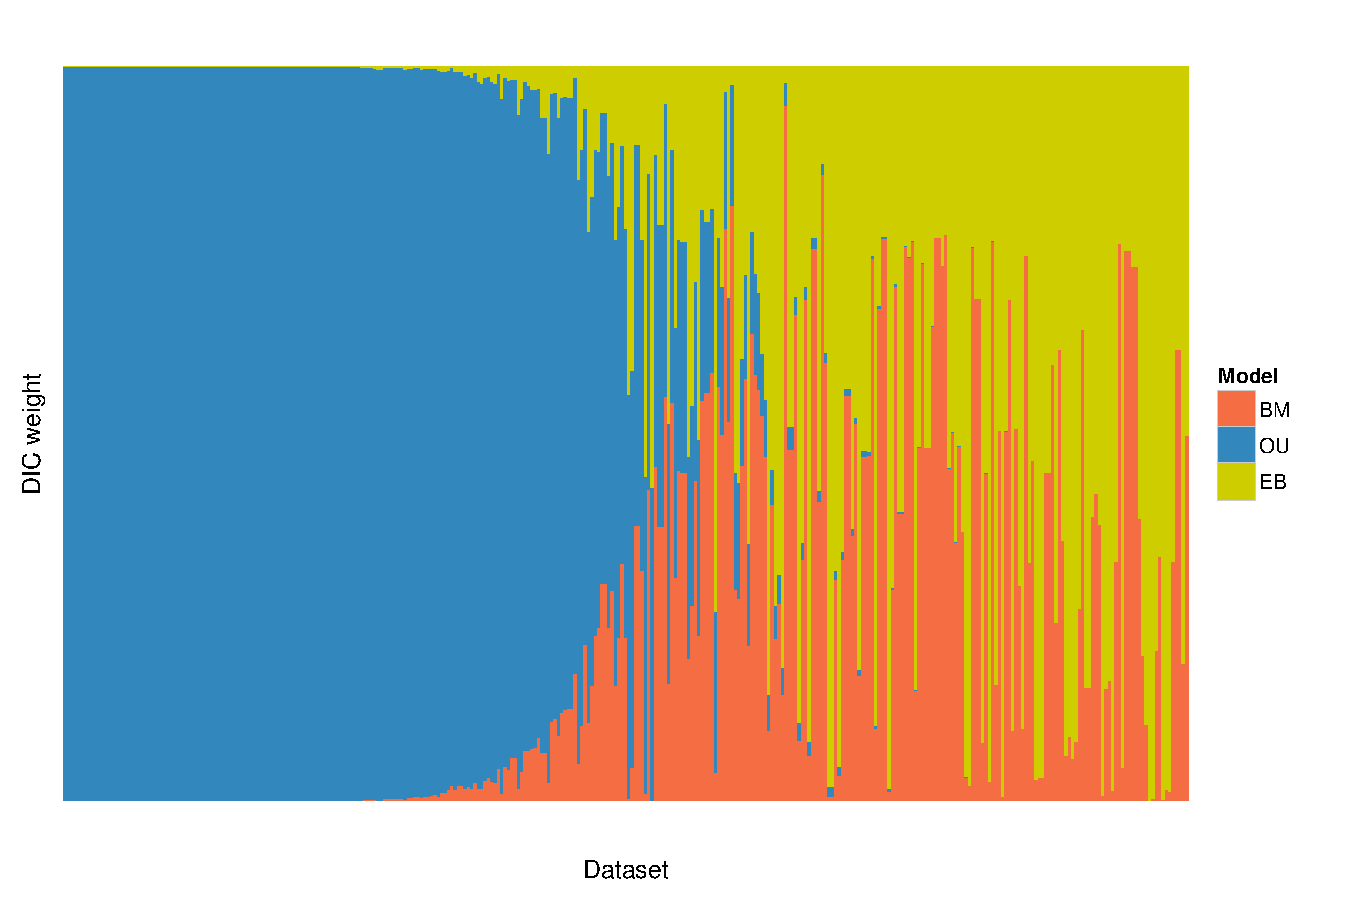
\includegraphics[angle=90, origin=c, scale=0.8]{figs/dic-support}
  \caption[Relative support for models across angiosperms (Bayesian)]{The relative support, as measured by DIC weight, for the three models used in our study (BM, OU, and EB) across all 337 datasets. All models were fit with MCMC. Like the model comparisons done with AIC, an OU model is highly supported for a majority of the datasets.}
  \label{fig:supp-dic-support}
\end{figure} 

For the model adequacy results, the results were also very similar to that of the likelihood analyses (compare to Results section in \spacedsmallcaps{Chapter 5}). The adequacy of these simple models was poor across the majority of the datasets (Figure \ref{fig:supp-pvalues}). Again, we limit our analyses of model adequacy to only the most highly supported model in the candidate set.

\begin{figure}[p]
  \centering
  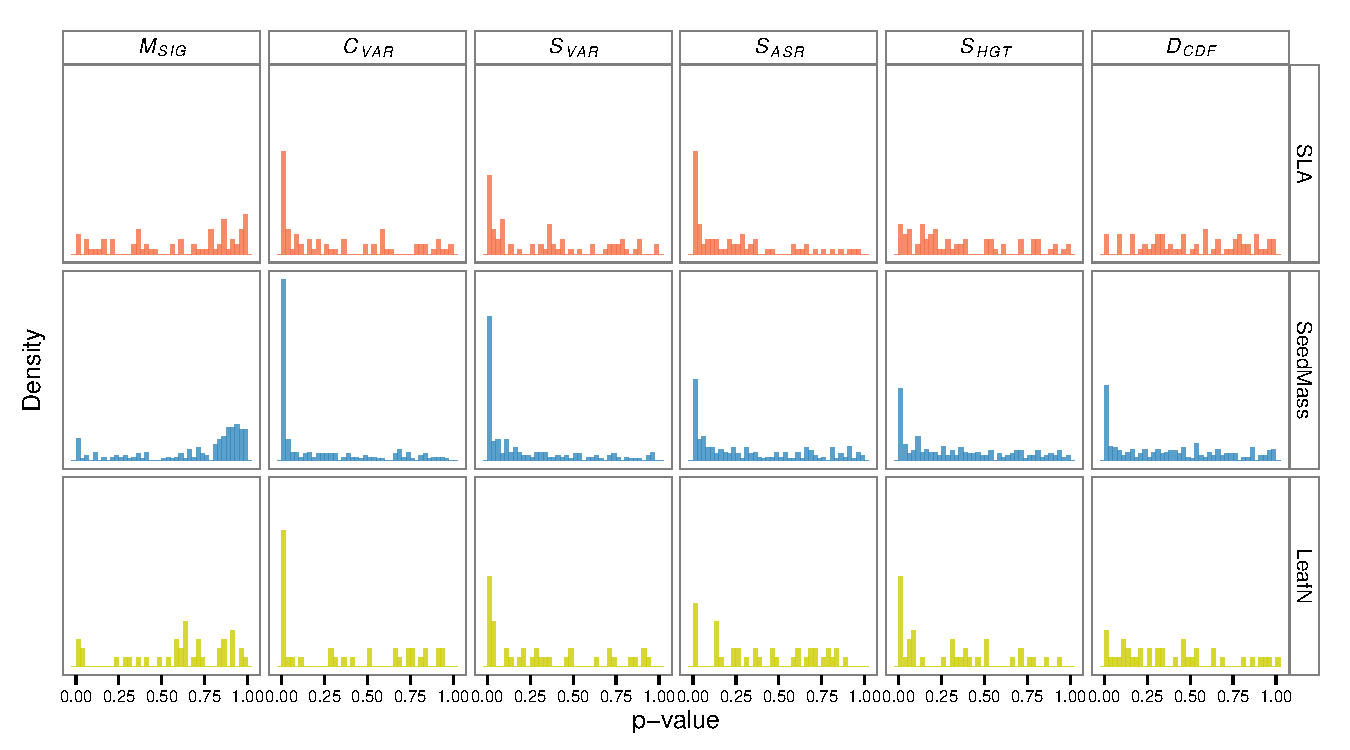
\includegraphics[angle=90, origin=c, scale=0.75]{figs/pval-hist-bayes}
  \caption[Distribution of $p$-values for all 337 datasets (Bayesian)]{The distribution of $p$-values for our six test statistics over all 337 datasets in our study after fitting the models using MCMC. The $p$-values are from applying our model adequacy approach to the best supported of the three models (as evaluated with DIC). Many of the datasets deviate from the expectations under the best model along a variety of axes of variation. Deviations are particularly common for the coefficient of variation $C_{\text{VAR}}$ and the slope of the contrasts against their expected variances $S_{\text{VAR}}$.}
  \label{fig:supp-pvalues}
\end{figure}


%% SLA data 
%% rejected by at least one ss: 35
%% rejected by at least two ss: 26
%% rejected by at least three ss: 19
Of the 72 comparative datasets of SLA, we detected deviations from the expectations of the best supported model using at least one test statistic in 35 cases, 26 by at least two, and 19 by three or more.
%% Seed mass data 
%% rejected by at least one ss: 173
%% rejected by at least two ss: 109
%% rejected by at least three ss: 72
For the seed mass data, we detected deviations with at least one test statistic in 173 cases (by two or more in 109 datasets and by at least three in 72 cases).
%% Leaf nitrogen data
%% rejected by at least one ss: 24
%% rejected by at least two ss: 13
%% rejected by at least three ss: 10
24/39 leaf nitrogen datasets were found to be inadequately described by the best supported model with at least one test statistic (13 by at least two and 10 by at least three).

%% Number rejected by each of the test statistics
%% m.sig: 24
%% c.var: 171
%% s.var: 141
%% s.asr: 101
%% s.hgt: 78
%% d.cdf: 67
Also, similar to the likelihood analyses, the frequency at which deviations were found differed between the test statistics. In 171 cases, we detected model misspecification with $C_{\text{VAR}}$ and with $S_{\text{VAR}}$, 141 ($M_{\text{SIG}}$: 24, $S_{\text{ASR}}$: 101, $S_{\text{HGT}}$: 78, $D_{\text{CDF}}$: 67). Again, only 105 datasets were adequately modeled by one of the three models in our candidate set. As with the likelihood analyses, we were more likely to detect model deviations when examining larger clades (figure \ref{fig:supp-size-adequacy}).

\begin{figure}[p]
  \centering
  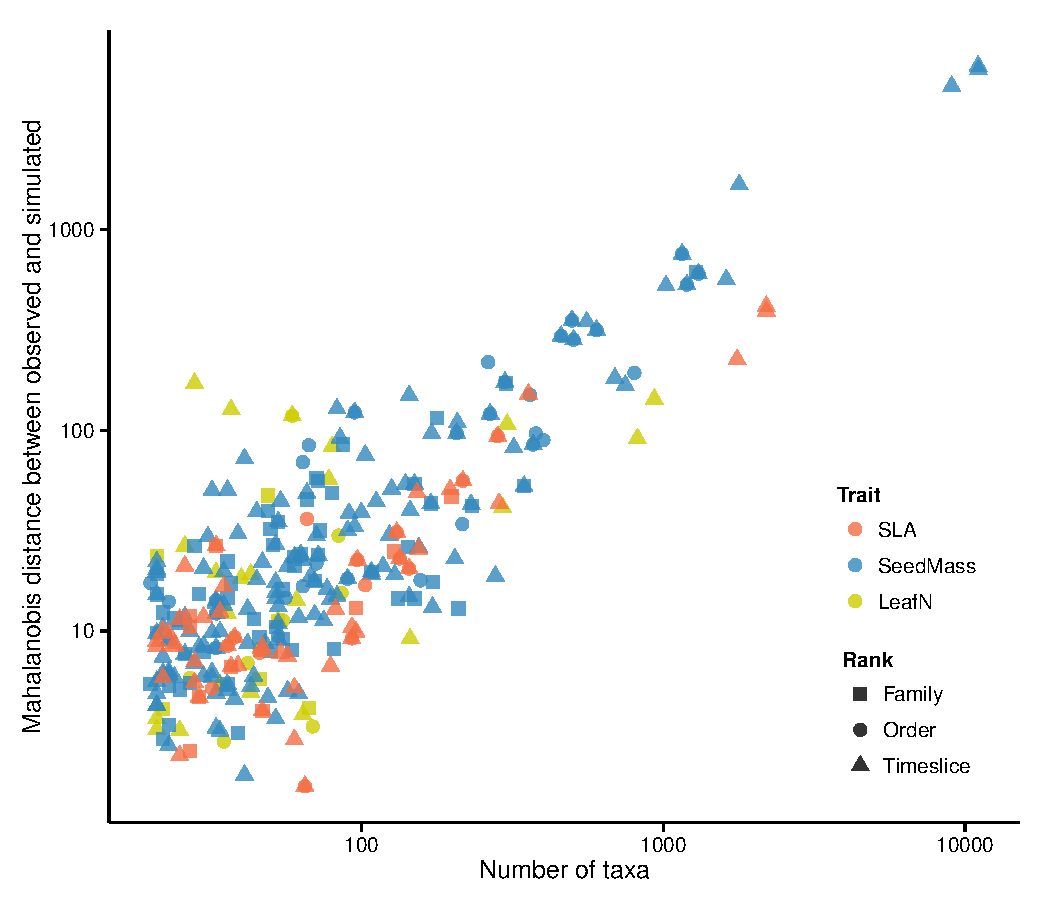
\includegraphics[width=\textwidth]{figs/ad-size-bayes}
  \caption[Model adequacy vs. clade size (Bayesian)]{The relationship between clade size and a multivariate measure of model adequacy from the Bayesian analysis. The Mahalanobis distance is a scale-invariant metric that measures the distance between the observed and simulated test statistics, taking into account the covariance between test statistics. The greater the Mahalanobis distance, the worse the model captures variation in the data. Considering only the best supported model for each clade (as chosen by DIC), there is a striking relationship between the two--the larger the dataset, the stronger the evidence that the model does not capture variation in the data.}
  \label{fig:supp-size-adequacy}
\end{figure}

